% SASYR 2025 - Template based on:
% samplepaper.tex, a sample chapter demonstrating the
% LLNCS macro package for Springer Computer Science proceedings;
% Version 2.20 of 2017/10/04
%
\documentclass[runningheads]{llncs}
%
\usepackage{graphicx}
\usepackage{subfigure}
\usepackage{amsmath}
\usepackage{lipsum}
\usepackage{url}
\usepackage[UTF8]{ctex}            %中文宏包
\usepackage{xcolor}                %字体颜色包
\usepackage[normalem]{ulem}        %支持删除线
\usepackage[dvipsnames]{xcolor}    %支持68种未预定义的颜色
\usepackage{float}                 %这三个包用于插入图片(后两个实现多张图片的并排插入)
\usepackage{enumerate}             %用于enumerate 列表中的自定义的标号
\usepackage[inline]{enumitem}      %内联列表,使列表嵌入文字中
\usepackage{tasks}                 %
\usepackage{amssymb}              %用于制考试选择题那样的水平列表
\usepackage{tabularx}
% Used for displaying a sample figure. If possible, figure files should
% be included in EPS format.
%
% If you use the hyperref package, please uncomment the following line
% to display URLs in blue roman font according to Springer's eBook style:
% \renewcommand\UrlFont{\color{blue}\rmfamily}

\begin{document}
\title{Lab3}
%
%\titlerunning{Abbreviated paper title}
% If the paper title is too long for the running head, you can set
% an abbreviated paper title here
%
\author{余俊洁 \orcidID{523030910244}}
%
\authorrunning{Augety}
% First names are abbreviated in the running head.
% If there are more than two authors, 'et al.' is used.
%
\institute{\email{YuJunjie-yjj@sjtu.edu.cn}}

\maketitle
\section{Control Logic}
\begin{itemize}
    \item 取址 (Fetch):
    \begin{itemize}
        \item 从当前 PC 所指内存中读取指令;
        \item PC 自增更新,准备下一条指令;
        \item 将指令转为二进制数组 command[16] 为后续译码做准备
    \end{itemize}
    \item 译码 (Decode):
    \begin{itemize}
        \item 将 command[16] 进行解码得到相应的 opcode.        
    \end{itemize}
    \item 执行 (Excute):
    \begin{itemize}
        \begin{table}[H]
            \centering 
            \begin{tabular}{|m{5cm}<{\centering}|m{2cm}<{\centering}|m{2cm}<{\centering}|}
            \hline
                \textbf{Operation} & \textbf{Opcode} & \textbf{Functions}\\ \hline
                ADD(2 ways) & 0001 (1) & ADD()\\ \hline
                AND(2 ways) & 0101 (5) & AND()\\ \hline
                BR & 0000 (0) & BR()\\ \hline
                JMP & 1100 (12) & JMP()\\ \hline
                JSR & 0100 (4) & JSR()\\ \hline
                LD & 0010 (2) & LD()\\ \hline 
                LDI & 1010 (10) & LDI()\\ \hline
                LDR & 0110 (6) & LDR()\\ \hline
                LEA & 1110 (14) & LEA()\\ \hline
                NOT & 1001 (9) & NOT()\\ \hline
                RET (achieved by JMP) & 1100 (12) & RET()\\ \hline
                RTI (not requested)& 1000 (8) & RTI()\\ \hline
                ST & 0011 (3) & ST()\\ \hline
                STI & 1011 (11) & STI()\\ \hline
                STR & 0111 (7) & STR()\\ \hline
                TRAP & 1111 (15) & TRAP()\\ \hline
            \end{tabular}
            \label{tabel.1}
        \end{table}
        \item 使用 switch-case 结构分发到不同的执行函数
    \end{itemize}
    \item 进行状态更新
\end{itemize}
\section{Important Functions}
\subsection{辅助函数}
\begin{enumerate}
    \item bin\_to\_dec(): 将一个位于 num[] 数组中、从 begin 到 end 的二进制位字段转换为一个十进制整数(支持补码)
    \item dec\_to\_bin(): 将一个十进制整数 n 转换成一个长度为 16 的二进制数组 res[],用于位级逻辑操作
    \item setNZP(): 根据寄存器或操作结果 num 的值,更新 LC-3 的条件码(N/Z/P)的值
\end{enumerate}
\subsection{操作函数: ADD(), BR(), LD(), $\cdots$}
 
\section{Verification}
为了检验各函数操作的正确性以及方便debug, 我写了一份包含了所有指令的一个汇编程序 `example.asm'
\begin{figure}[H]
    \centering
    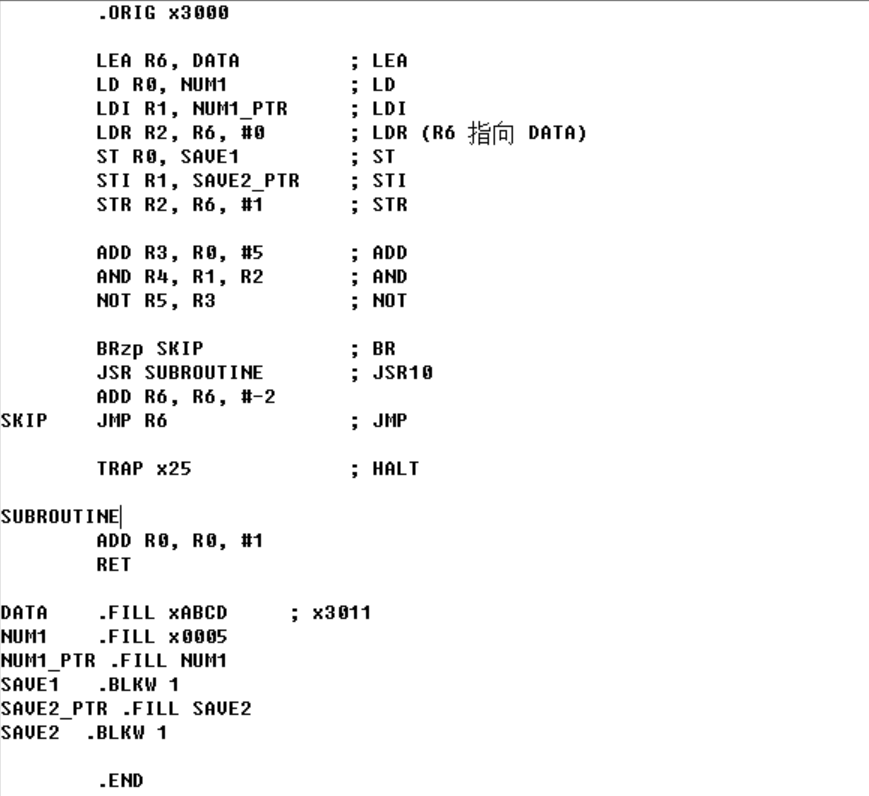
\includegraphics[width=0.8\textwidth]{1.png}
    \caption{example.asm}
    \label{fig:3-1}
\end{figure}
同时,为了验证正确性,我不仅会直接根据example.asm分析运行的结果进行验证,还将通过将我的simulater运行的结果与我在windows主机上安装官方的simulater在各个断点运行的结果相对比.
\begin{figure}[H]
    \centering
    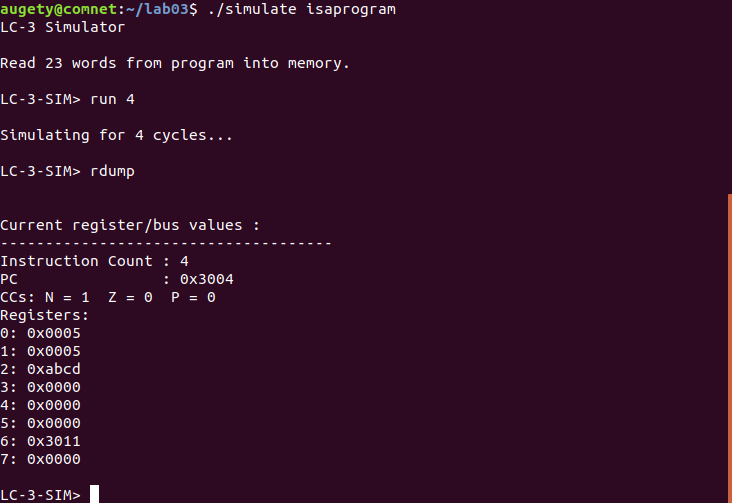
\includegraphics[width=0.75\textwidth]{2.png}
    \label{fig:3-2}
    \caption{LD系列操作}
\end{figure}
\vspace{-1.5cm}
\begin{figure}[H]
    \centering
    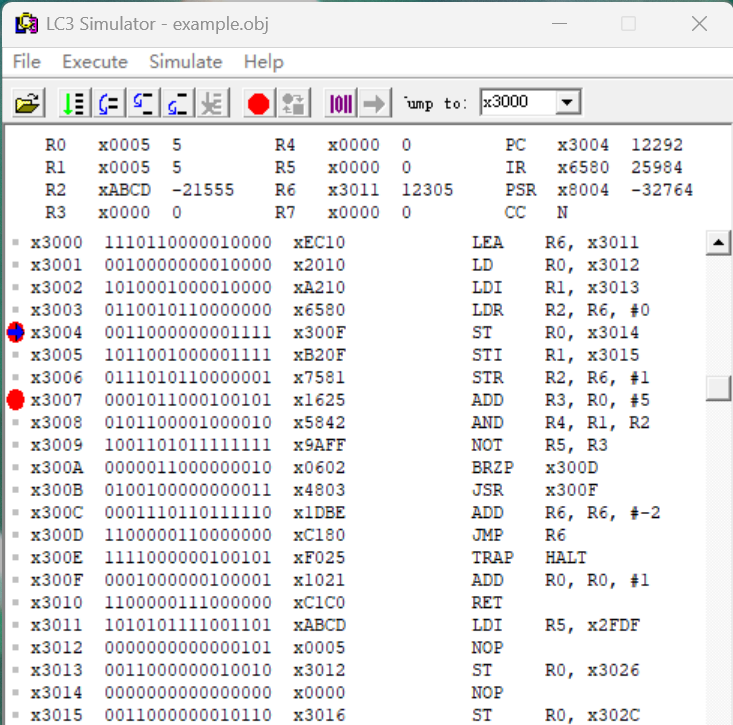
\includegraphics[width=0.7\textwidth]{3.png}
    \caption{LD系列操作}
    \label{fig:3-3}
\end{figure}
在执行x3000到x3003的四条不同的LD指令之后,我的simulator和官方的得到的各个寄存器的值保持一致,证明了我的simulator对于LEA,LD,LDI,LDR指令实现的正确性。

具体来说,通过LEA指令,我们将DATA标签的地址也就是x3011存进了R6;通过LD指令,将NUM1的值也就是x0005存进R0;通过LDI指令,将NUM1\_PTR指向的值(NUM1)作为地址对应的值x0005存入R1;通过LDR指令,将R6存的值作为地址(x3011)指向的值xABCD存入R2. 经检验,得到的结果均符合我们的分析。
\begin{figure}[H]
    \centering
    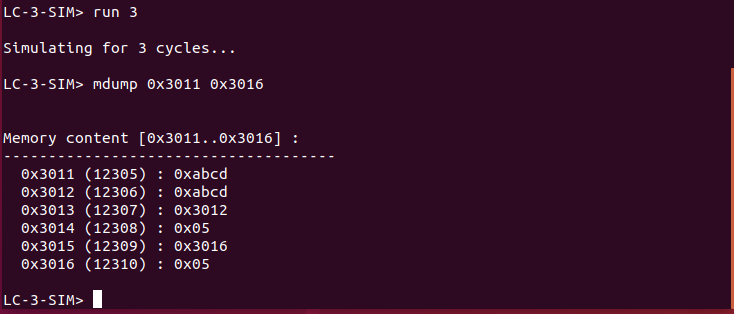
\includegraphics[width=0.75\textwidth]{4.png}
    \caption{ST系列操作}
    \label{fig:3-4}
\end{figure}
\vspace{-1cm}
\begin{figure}[H]
    \centering
    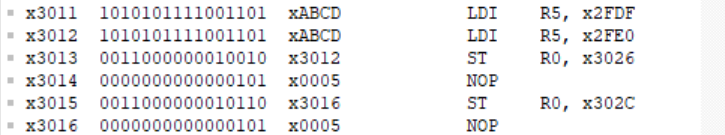
\includegraphics[width=0.7\textwidth]{5.png}
    \caption{ST系列操作}
    \label{fig:3-5}
\end{figure}
在执行x3004到x3006的三条不同的ST指令之后,我的simulator和官方的得到的对应的地址内存入的值保持一致,证明了我的simulator对于ST,STI,STR指令实现的正确性。

具体来说,通过ST指令,我们将R0的值存在了SAVE1对应的地址(x3010);通过STI指令,我们将R1的值存在了SAVE2\_PTR对应的值对应的地址,也即是SAVE2的位置(x3016);通过STR指令,我们将R2的值,存在了R6的值+1对应的地址,也即NUM1的位置(x3012). 经检验,得到的结果均符合我们的分析。
\begin{figure}[H]
    \centering
    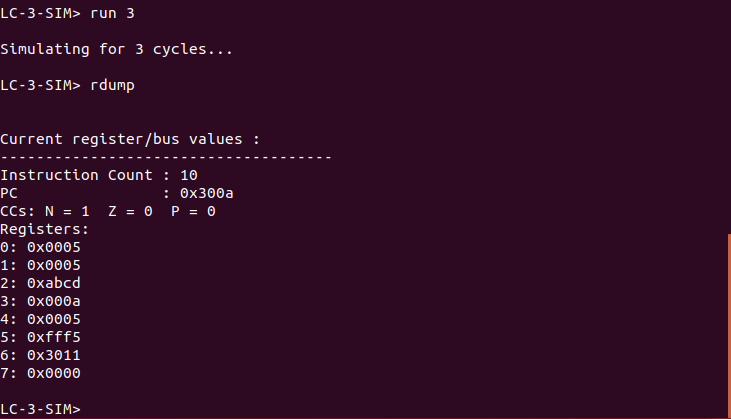
\includegraphics[width=0.75\textwidth]{6.png}
    \caption{运算系列操作}
    \label{fig:3-6}
\end{figure}
\vspace{-1cm}
\begin{figure}[H]
    \centering
    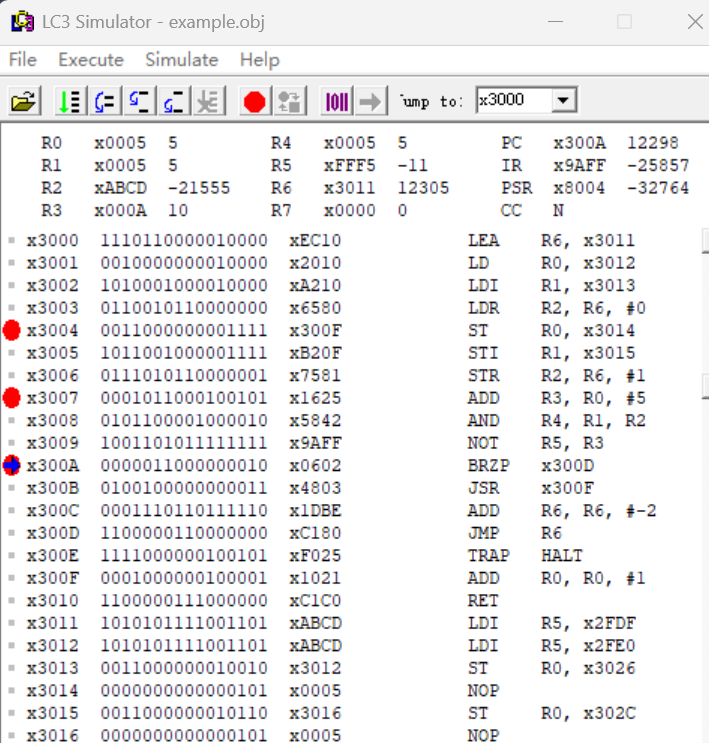
\includegraphics[width=0.7\textwidth]{7.png}
    \caption{运算系列操作}
    \label{fig:3-7}
\end{figure}
在执行x3007到x3009的三条不同的运算指令之后,我的simulator和官方的得到的各个寄存器的值保持一致,证明了我的simulator对于ADD,AND,NOT指令实现的正确性。
同时,也易分析该结果的正确性。
\begin{figure}[H]
    \centering
    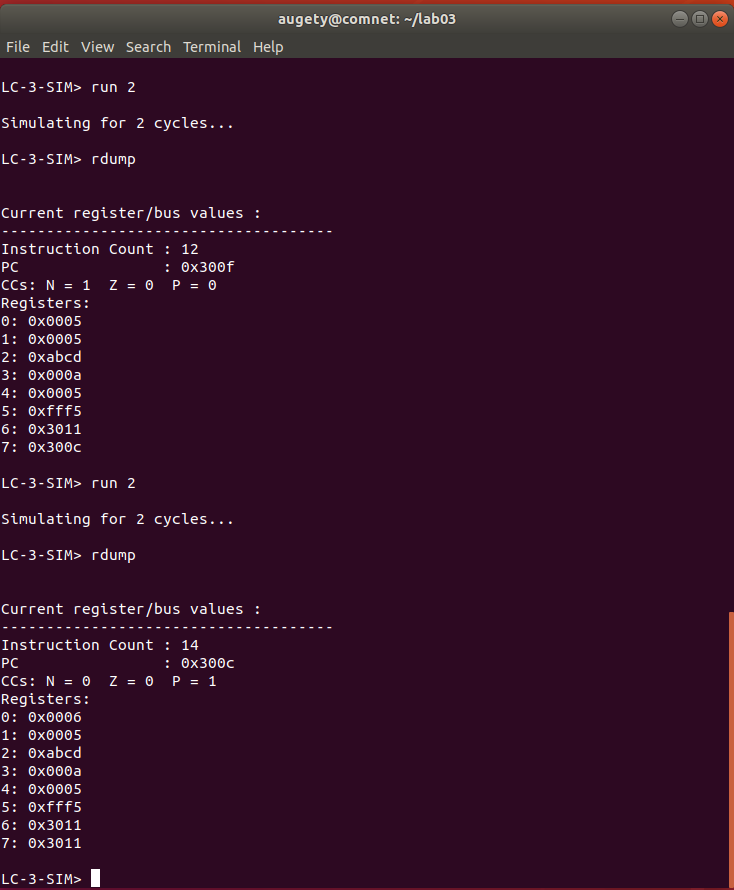
\includegraphics[width=0.6\textwidth]{8.png}
    \caption{JSR操作}
    \label{fig:3-8}
\end{figure}
\vspace{-1cm}
\begin{figure}[H]
    \centering
    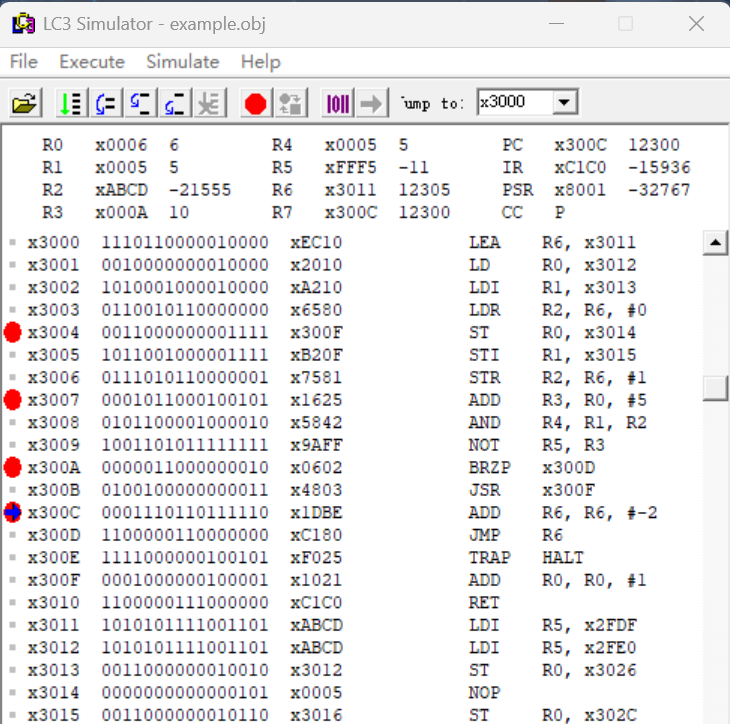
\includegraphics[width=0.6\textwidth]{9.png}
    \caption{JSR操作}
    \label{fig:3-9}
\end{figure}
由于执行完NOT指令, $N=1$,故BR指令不执行跳转,此处simulator也确实没有跳转,可得对于BR指令的正确性;接着执行JSR指令跳转到SUBROUTINE,执行完$R0 + 1$的操作之后返回原程序。故此时PC=0x300c, R0 = x0006。得到的结果与分析一致,也与官方的simulator一致。可得对于JSR指令的正确性。
\vspace{-0.6cm}
\begin{figure}[H]
    \centering
    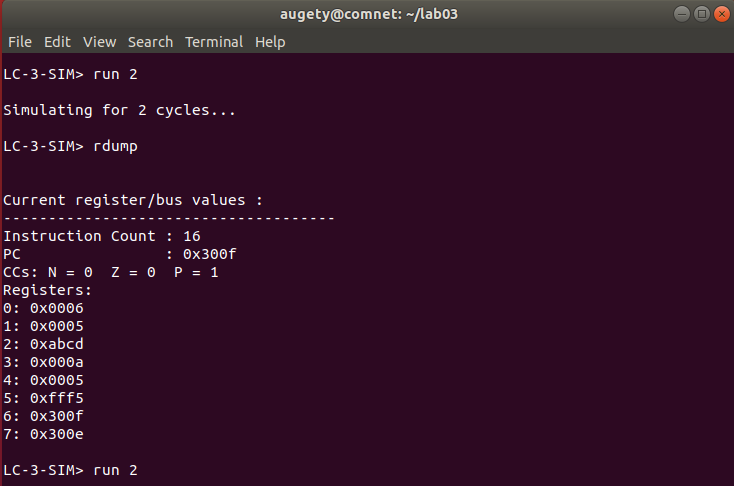
\includegraphics[width=0.6\textwidth]{10.png}
    \caption{JMP操作}
    \label{fig:3-10}
\end{figure}
\vspace{-1.2cm}
\begin{figure}[H]
    \centering
    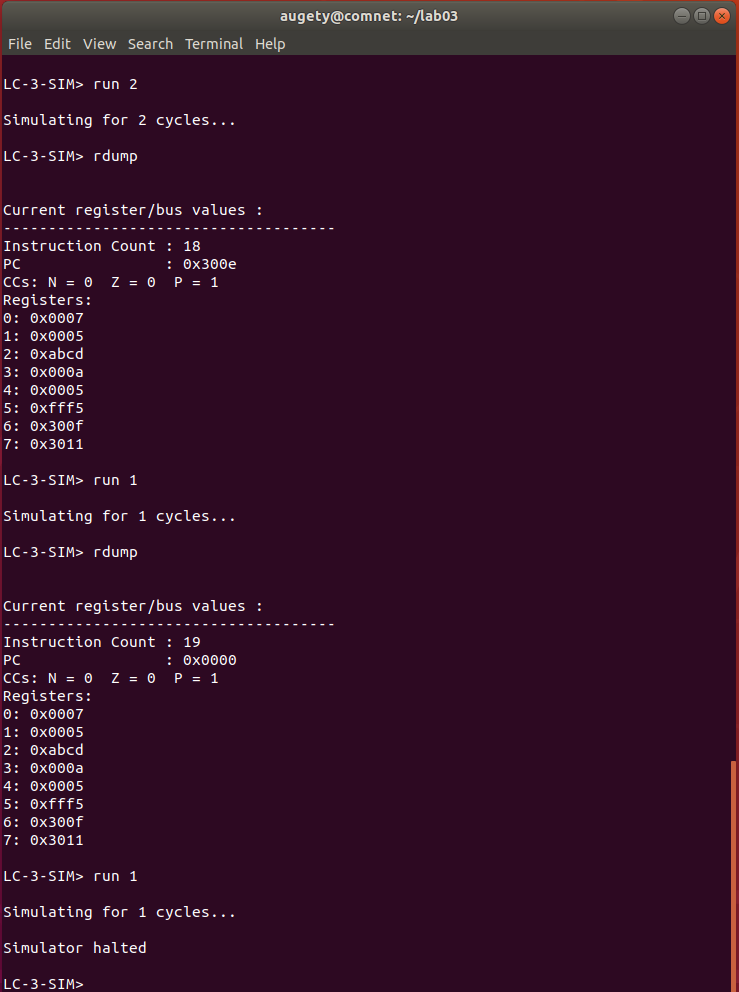
\includegraphics[width=0.55\textwidth]{11.png}
    \caption{TRAP操作}
    \label{fig:3-11}
\end{figure}
当我们再run两步执行JMP指令,再一次跳到SUBROUTINE子进程,此时PC的值为x300F,与得到的结果一致,当我们再执行两步之后,此时的PC的值为x300E,又跳回了原程序并将要执行TRAP x25指令终止程序,符合实验结果。当我们再执行一步,即为执行TRAP x25指令,此时按照题目要求,我们需要将PC置为0,进而终止程序运行,也与我们的实验结果想吻合。由此可得simulator对于JMP指令和TRAP指令的正确性。

由此,通过对于每一个操作指令的验证之后,我们可以验证我所编写的simulator的完备性与正确性。
\bibliographystyle{refs-style}
\bibliography{refs}
\end{document}
